% --------------------------------------------------------------
% This is all preamble stuff that you don't have to worry about.
% Head down to where it says "Start here"
% --------------------------------------------------------------
 
\documentclass[12pt]{article}

\usepackage{courier}
\usepackage{color}
\usepackage{listings}
\usepackage[square,numbers]{natbib}
\usepackage{tabls}
\usepackage{graphicx}
\usepackage{subcaption}
\usepackage{pdfpages}
\usepackage{mathtools}

\definecolor{dkgreen}{rgb}{0,0.6,0}
\definecolor{gray}{rgb}{0.5,0.5,0.5}




\lstset{language=Matlab,
   keywords={break,case,catch,continue,else,elseif,end,for,function,
      global,if,otherwise,persistent,return,switch,try,while},
   basicstyle=\ttfamily,
   keywordstyle=\color{blue},
   commentstyle=\color{red},
   stringstyle=\color{dkgreen},
   numbers=left,
   numberstyle=\tiny\color{gray},
   stepnumber=1,
   numbersep=10pt,
   backgroundcolor=\color{white},
   tabsize=4,
   showspaces=false,
   showstringspaces=false}
 
\usepackage[margin=1in]{geometry} 
\usepackage{amsmath,amsthm,amssymb}
\usepackage{verbatim}
\usepackage{algpseudocode,algorithm}
\usepackage{setspace}

\newcommand{\lline}{\noindent\makebox[\linewidth]{\rule{\textwidth}{0.4pt}}}
\newcommand{\N}{\mathbb{N}}
\newcommand{\Z}{\mathbb{Z}}
\newcommand{\deriv}[2]{\frac{\mathrm{d} #1}{\mathrm{d} #2}}
\newcommand{\pderiv}[2]{\frac{\partial #1}{\partial #2}}
\newcommand{\bx}{\mathbf{X}}
\newcommand{\ba}{\mathbf{A}}
\renewcommand{\d}{\mathrm{d}}
\newcommand{\upl}{u_{\text{plane}}}
\newcommand{\upt}{u_{\text{point}}}
\newcommand{\D}{\Delta}
\newcommand{\ra}{\rightarrow}
\renewcommand{\SS}{\State}
 
\newenvironment{theorem}[2][Theorem]{\begin{trivlist}
\item[\hskip \labelsep {\bfseries #1}\hskip \labelsep {\bfseries #2.}]}{\end{trivlist}}
\newenvironment{lemma}[2][Lemma]{\begin{trivlist}
\item[\hskip \labelsep {\bfseries #1}\hskip \labelsep {\bfseries #2.}]}{\end{trivlist}}
\newenvironment{exercise}[2][Exercise]{\begin{trivlist}
\item[\hskip \labelsep {\bfseries #1}\hskip \labelsep {\bfseries #2.}]}{\end{trivlist}}
\newenvironment{problem}[2][Problem]{\begin{trivlist}
\item[\hskip \labelsep {\bfseries #1}\hskip \labelsep {\bfseries #2:}]\hspace{0.3in}\newline\newline}{\end{trivlist}}
\newenvironment{question}[2][Question]{\begin{trivlist}
\item[\hskip \labelsep {\bfseries #1}\hskip \labelsep {\bfseries #2.}]}{\end{trivlist}}
\newenvironment{corollary}[2][Corollary]{\begin{trivlist}
\item[\hskip \labelsep {\bfseries #1}\hskip \labelsep {\bfseries #2.} ]}{\end{trivlist}}
\newenvironment{problem*}[1][Problem]{\begin{trivlist}
\item[\hskip \labelsep {\bfseries #1} {\hspace{-0.2em}\bfseries:}]}{\end{trivlist}}
\newenvironment{solution}[1][Solution]{\begin{trivlist}
\item[\hskip \labelsep {\bfseries #1} {\hspace{-0.2em}\bfseries:}]\hspace{0.3in}\newline}{\end{trivlist}}
 
\begin{document}
 
% --------------------------------------------------------------
%                         Start here
% --------------------------------------------------------------
 
\title{Homework 1}%replace X with the appropriate number
\author{Simon Bolding\\ %replace with your name
NUEN 629} %if necessary, replace with your course title
 
\maketitle

\clearpage

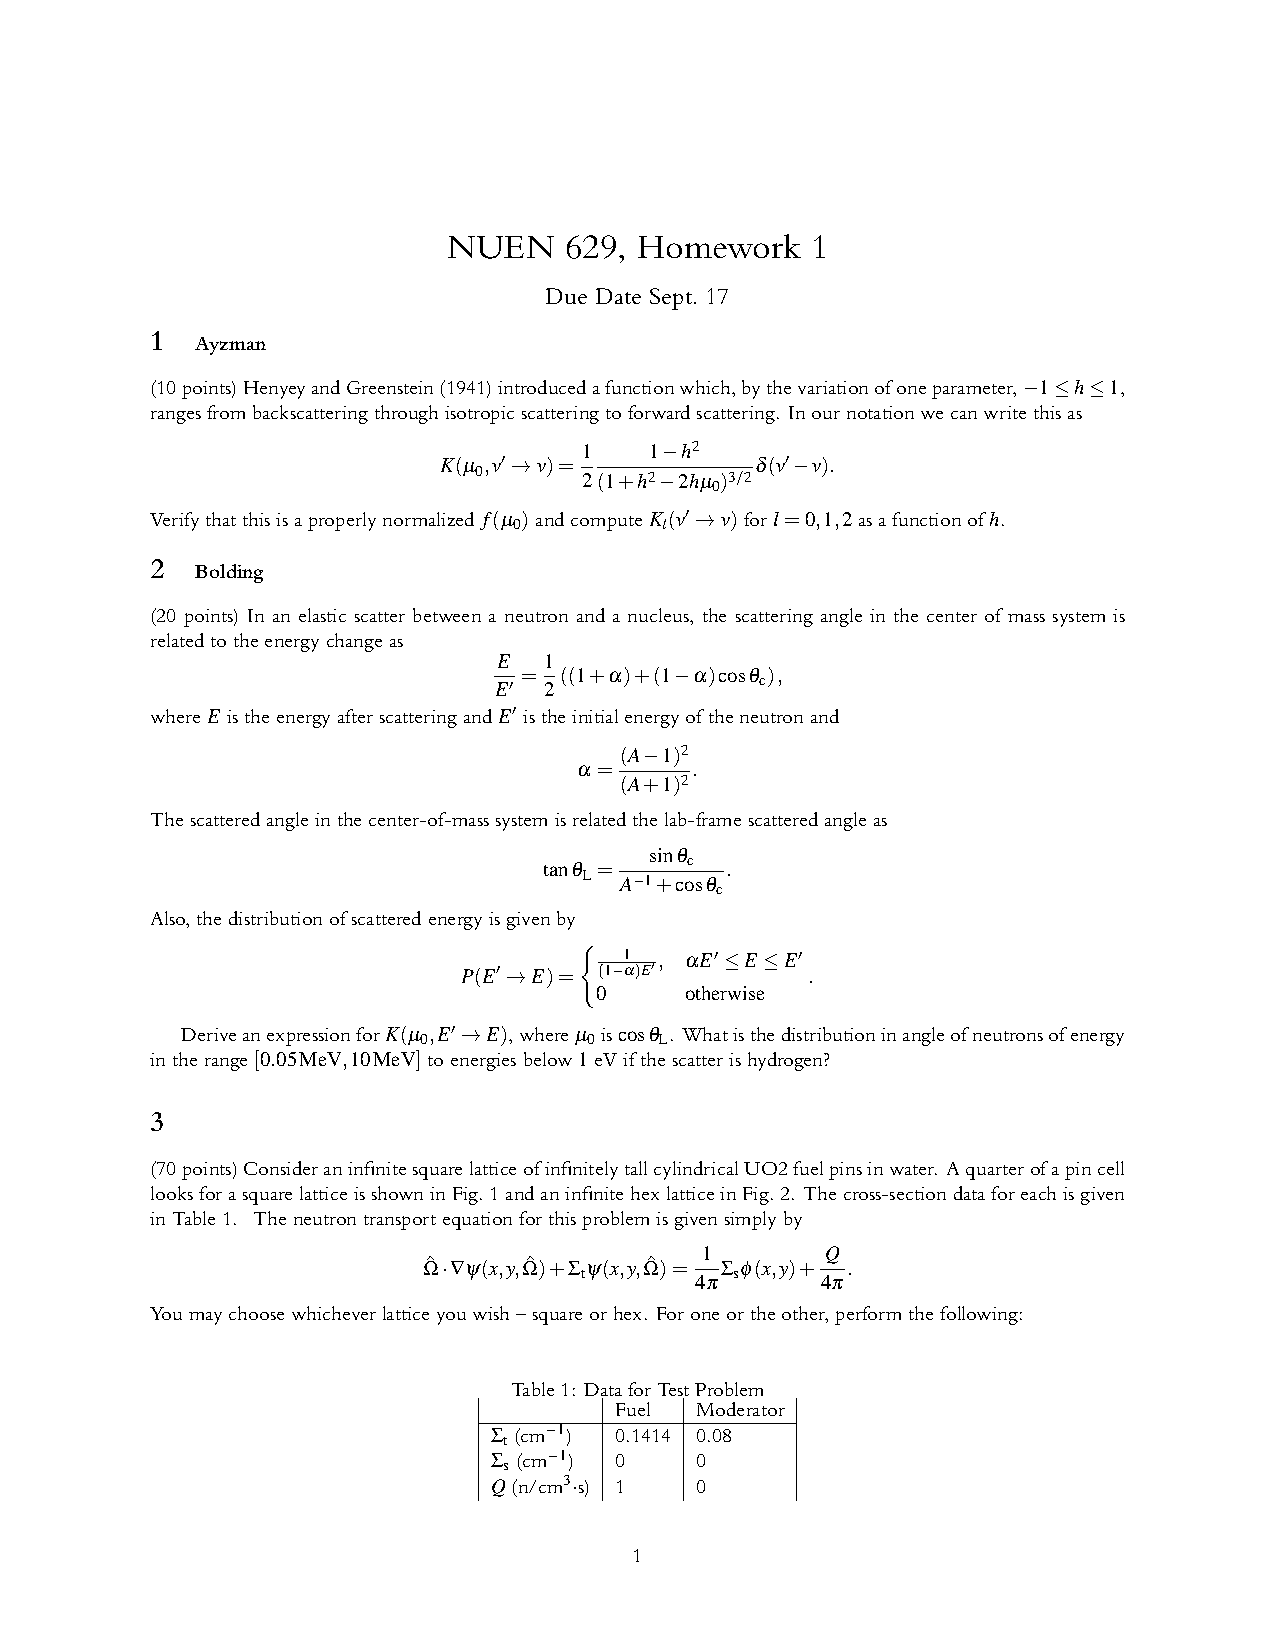
\includepdf[pages={1-3}]{Homework1.pdf}

%\includepdf[pages={1}]{p1p3.pdf}

\begin{problem}{1}
Henyey and Greenstein (1941) introduced a function which, by the variation of one
parameter, $−1 \leq h \leq 1$, ranges from backscattering through isotropic scattering to forward scattering. In
our notation we can write this as
\begin{equation}
    K( \mu_0 , v'\rightarrow v) = \frac{1}{2}
    \frac{1-h^2}{\left(1+h^2-2h\mu_0\right)^{3/2}}\delta(v'-v).
\end{equation}
Verify that this is a properly normalized $f ( \mu_0 )$ and compute $K_l (v'
\rightarrow → v)$ for $l = 0, 1, 2$ as a function of $h$.

\end{problem}

\begin{solution}
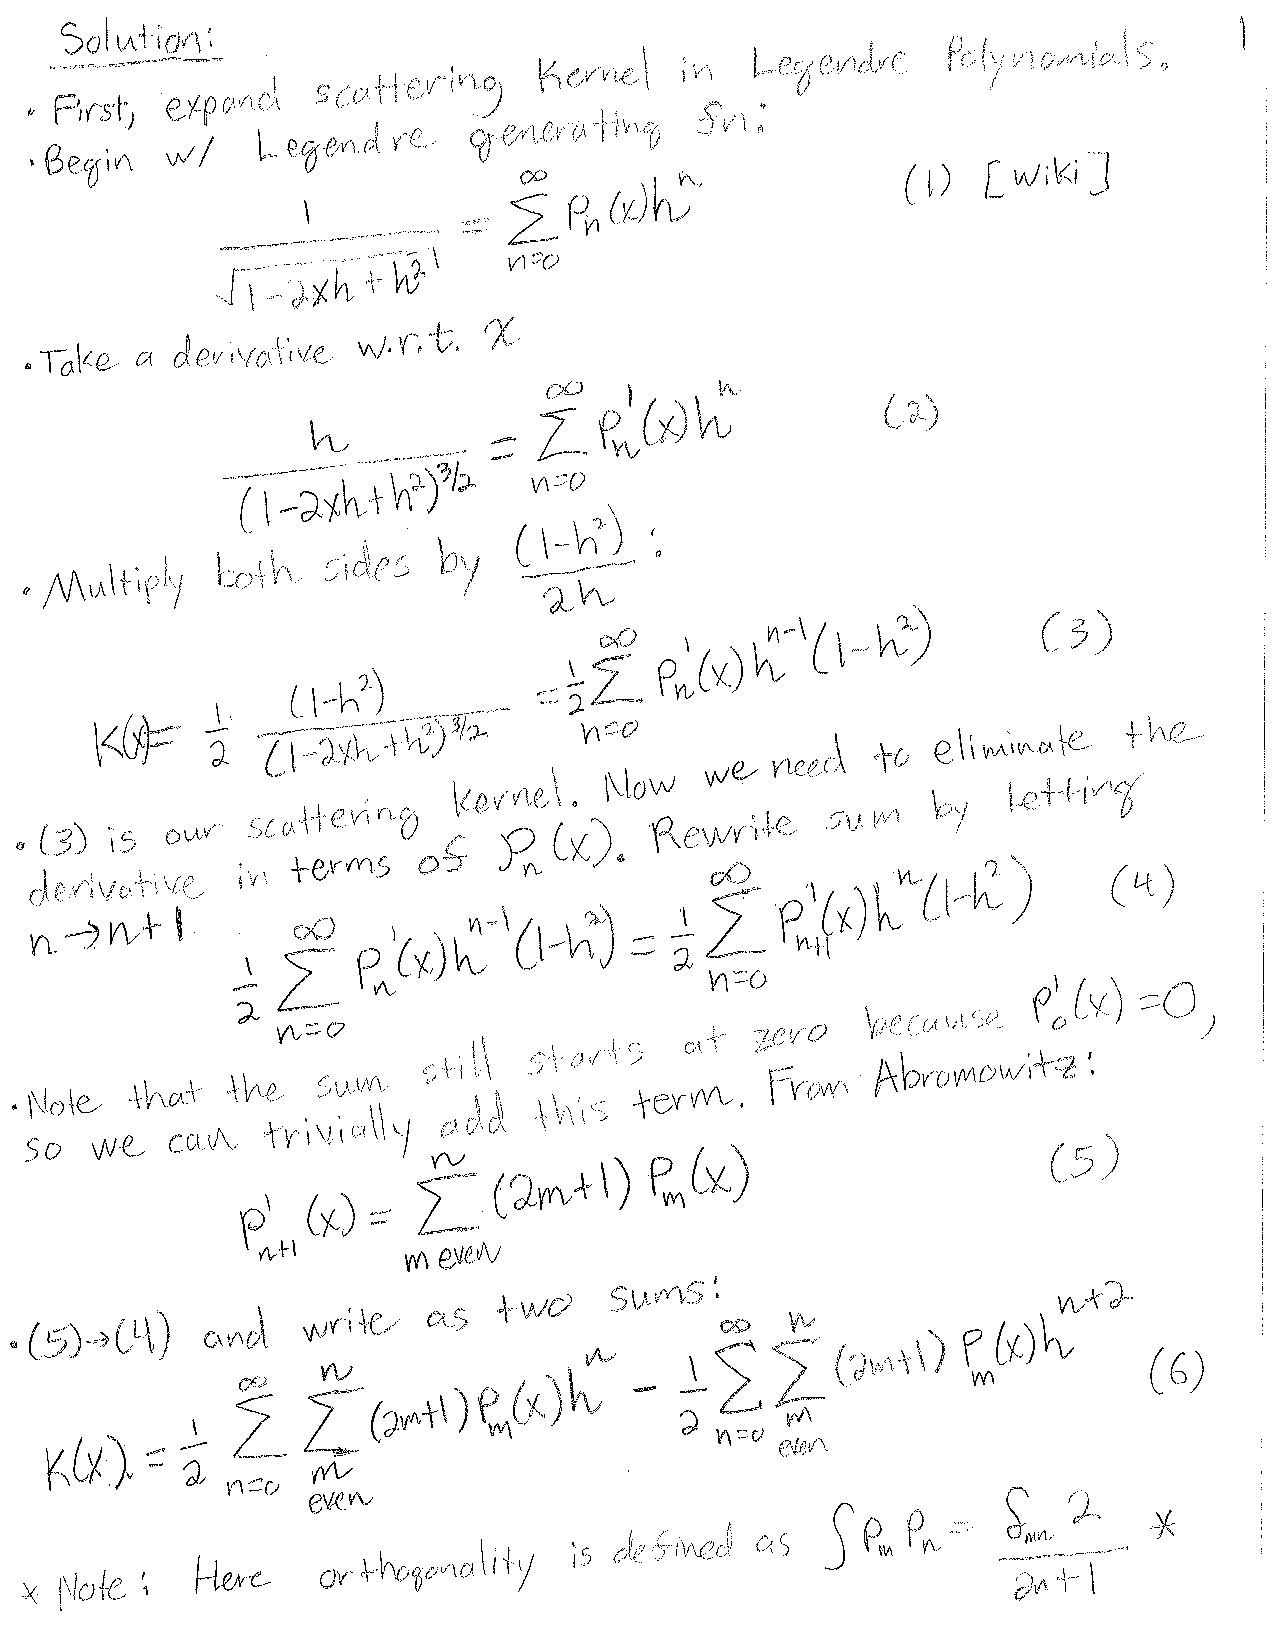
\includepdf[pages={1-2}]{p1.pdf}
\end{solution}
\clearpage

\begin{problem}{2}
In an elastic scatter between a neutron and a nucleus, the scattering angle in the center of mass system is
related to the energy change as
\begin{equation}\label{eq:E}
 \frac{E}{E'} = \frac{1}{2}\left((1+\alpha) + (1-\alpha)\cos \theta_c\right)
\end{equation}
where $E$ is the energy after scattering and $E'$′ is the initial energy of the neutron and
\begin{equation}
\alpha = \frac{(A-1)^2}{(A+1)^2}.
\end{equation}
The scattered angle in the center-of-mass system is related the lab-frame scattered angle as
\begin{equation}\label{eq:tan}
\tan \theta_L = \frac{A\sin \theta_c}{1 + A\cos \theta_c}
\end{equation}
Also, the distribution of scattered energy is given by
\begin{equation} \label{pdf}
P(E'\rightarrow E) = \left\{\begin{matrix}
\frac{1}{(1-\alpha)E'} & E'\alpha \leq E \leq E' \\ 
 0 & \text{otherwise}
\end{matrix}\right. .
\end{equation}
Derive an expression for $K( \mu_0, E'\rightarrow E)$, where $\mu_0$ is $\cos \theta_L$. What is the distribution in angle of neutrons of energy
in the range [0.05 MeV, 10 MeV] to energies below 1 eV if the scatter is with hydrogen?

\end{problem}

\begin{solution}

    \subsubsection*{Scattering Kernel Derivation}

Due to Eq.~\eqref{eq:E}, for a fixed $A$, a given value of $E$ and $E'$ fully define
$\mu_c$; the lab frame cosine of the scattering angle $\mu_0$ is also fully defined through
Eq.~\eqref{eq:tan}.  As a result, the shape of the doubly differential scattering cross section
 is fully defined by the probability density function (PDF) $P(E'\ra E)$. Thus, it is
possible to write the scattering cross section in the COM frame as~\cite{dunnshultis}
\begin{equation}
    \Sigma_s(\mu_0,E'\ra E) = \Sigma_s(E')P(E' \ra E) \delta(\mu_c - f_\mu(E,E'))
 \end{equation}
 where $f_\mu(E,E')$ is the value of $\mu_c$ that satisfies Eq.~\eqref{eq:E} for a given
 $E$, i.e.,
 \begin{equation}
     f_\mu(E,E') = \frac{2(\frac{E}{E'}) - (1+\alpha)}{(1-\alpha)}
 \end{equation}
Because we are interested in the scattering kernel as a function of the lab frame
cosine $\mu_0$, 
we define the scattering cross section in an equivalent form 
 \begin{equation}
     \Sigma_s(\mu_0,E'\ra E) = \Sigma_s(E')P(\mu_0)\delta(E - f_{E}(\mu_c(\mu_0),E'))
 \end{equation}
 where $P(\mu_0)$ is a PDF for $\mu_0$ given a certain value of $E'$, $f_E$ is
 defined as
 \begin{equation}
  f(\mu_0,E') = \frac{E'}{2}\left((1+\alpha) + (1-\alpha)\mu_c\right),
 \end{equation}
 and $\mu_c$ as a function of $\mu_0$ will be derived later in Eq.~\eqref{eq:muc}. The scattering kernel is defined as
 \begin{equation}
     K(\mu_0,E'\ra E) = \frac{\Sigma_s(E'\ra E,\mu_0)}{\displaystyle\int\limits_{0}^\infty\d
     E\!\int\limits_{-1}^1 \d \mu_0\,
 \Sigma_s(E'\ra E,\mu_0)}
 \end{equation}
 The denominator is evaluated as
 \begin{equation}
     \int\limits_{-1}^1 \!\d \mu_0 \int\limits_0^\infty \!\d E \;
     \Sigma_s(E')P(\mu_0)\delta(E-f_{E}(\mu_c(\mu_0),E)) =
     \Sigma_s(E')\int\limits_{-1}^1 \d\mu_0 P(\mu_0) = \Sigma_s(E')
 \end{equation}
 where the first equality is true because the argument of the delta function is zero
 for the value of $\mu_0$ and $E'$ that satisfy $f$, which in this case gives the
 $\mu_0$ that is the integration variable of the
 outer integral.  The scattering Kernel is then just
 \begin{equation}
     K(\mu_0,E'\ra E) = P(\mu_0)\delta(E - f_{E}(\mu_C(\mu_0),E)).  
 \end{equation}
 We now need to transform the PDF $P(E'\ra E)$ into a density function
 $P(\mu_0)$.  From Eq.~\eqref{eq:E},
 there is a one-to-one relationship between $E$ and $\mu_c=\cos(\Theta_c)$ in the
 range of $E\in[\alpha E',E']$, thus
 \begin{equation}
  P(E'\ra E) \d E = P(\mu_c)\d \mu_c
 \end{equation}
or
 \begin{equation} \label{pdfmu}
     P(\mu_c) = P(E' \ra E) \frac{\d E}{\d \mu_c} .
 \end{equation}
 Multiplication of Eq.~\eqref{eq:E} by $E'$, followed by differentiation, yields
 \begin{equation}
     \frac{ \d E}{\d \mu_c} = \frac{1}{2}(1-\alpha) E'
 \end{equation}
 Evaluating $\mu_c$ for $E$ at the limits $\alpha E'$
 and $E'$ gives the support for $P(\mu_c)$, defined for $\mu_c \in[ -1,1 ]$.  
 Substitution of the above equation and Eq.~\eqref{pdf} into Eq.~\eqref{pdfmu} gives
 the PDF in the COM frame
 \begin{equation}\label{eq:pdfc}
     P(\mu_c) = \frac{1}{(1-\alpha)E'} \left( \frac{1}{2}(1-\alpha)E' \right) =
     \frac{1}{2}, \quad \mu_c \in [-1,1]
 \end{equation}
 We must now transform to the lab frame scattering cosine $\mu_0$.  First, we solve
 Eq.~\eqref{eq:tan} for $\mu_0$ in terms of $\mu_c$ as follows:
 \begin{align}
  \tan^2\theta_L &= \left(\frac{A\sin \theta_c}{1 + A\cos \theta_c}\right)^2 \\
  \sec^2\theta_L - 1&= \left(\frac{A\sin \theta_c}{1 + A\cos \theta_c}\right)^2\\
  \mu_0^{-2} &= \frac{A^2(\sin^2\theta_c + \cos^2\theta_c) + 1 + 2A\mu_c}{\left(1+A\mu_c\right)^2}\\
  \mu_0 &= \frac{1+A\mu_c}{\sqrt{1+2\mu_cA+A^2}}. \label{eq:mul}
 \end{align}
Solution of the above equation for $\mu_c$ in terms of $\mu_L$ gives
\begin{equation}\label{eq:muc}
    \mu_c = -\frac{1}{A}(1-\mu_0^2) + \mu_0\sqrt{1-\frac{1}{A^2}(1-\mu_0^2)}\;.
\end{equation}
Eq.~\eqref{eq:mul} demonstrates a one-to-one relationship between $\mu_0$ and
$\mu_C$.  As before,
\begin{equation}\label{eq:pdfle}
P(\mu_0) = P\left(\mu_C(\mu_0)\right)\frac{\d \mu_c}{\d \mu_0}.
\end{equation}
Differentiation of Eq.~\eqref{eq:muc} with respect to $\mu_0$ and algebraic
manipulation ultimately yields
\begin{equation}
    \frac{\d \mu_c}{\d \mu_0} = \frac{2 \mu_0}{A} + \frac{1 - \frac{1}{A^2}(1 -
2\mu_0^2)}{\sqrt{1 - \frac{1}{A^2}(1 - \mu_0^2)}}.
\end{equation}
Substitution of the above equation and Eq.~\eqref{eq:pdfc} into Eq.~\eqref{eq:pdfle}
gives an expression for $P(\mu_0)$. The final expression for the scattering kernal
is, for $A>1$
\begin{equation}
    \boxed{
K(\mu_0,E'\rightarrow E) = \left\{\begin{matrix} \displaystyle
\left[\frac{\mu_0}{A} + \frac{1 - \frac{1}{A^2}(1 -
2\mu_0^2)}{2\sqrt{1 - \frac{1}{A^2}(1 -
\mu_0^2)}}\right]{\delta(E-f_E\left(\mu_c(\mu_0),E'\right))}, & \mu_0\in[-1,1] \\ 
 0, & \text{otherwise}
\end{matrix}\right. 
}.
\end{equation}
where the support is from evaluation of Eq.~\eqref{eq:mul} at $\mu_c=-1,1$.  The case
of $A=1$ must be treated separately. This can be seen, for instance, because evaluation of
Eq.~\eqref{eq:mul} at $\mu_c=-1$ results in an indeterminant $0/0$. Evaluation of
Eq.~\eqref{eq:muc} for $A=1$ gives a non-indeterminant expression for $\mu_0$ as
\begin{equation}\label{eq:mu0}
    \mu_0 = \sqrt{\frac{1+\mu_c}{2}}
\end{equation}
Thus, the support becomes $\mu_0 \in [0,1]$.  The kernel also simplifies significantly at
$A=1$.  The final scattering kernel, for the case of $A=1$, is
\begin{equation}\label{answer}
\boxed{
K(\mu_0,E'\rightarrow E) = \left\{\begin{matrix}
2\mu_0\delta(E-f_E\left(\mu_c(\mu_0),E'\right)), & \mu_0\in[0,1] \\ 
 0, & \text{otherwise}
\end{matrix}\right. 
}.
\end{equation}
which is PDF normalized over $\mu_0$ and $E$.

\subsubsection*{Plots for A=1}

To plot in terms of energy, we evaluate Eq.~\eqref{eq:E} at $A=1$, giving
\begin{equation}
    \frac{E}{E'} = \frac{1+\mu_c}{2}.
\end{equation}
Then, using Eq.~\eqref{eq:mu0}, $\mu_0$ in terms of $E$ and $E'$ is 
\begin{equation}
    \mu_0 = \sqrt{\frac{E}{E'}}.
\end{equation}
A plot of $P(\mu_0)$ vs $\mu_0$ and $P(\mu(E',E))$ vs $E'$ are given below.  The
values of $E'$ range between
$0.05$ MeV to $10$ MeV, with $E$ fixed at 1 eV.  As expected, lower energy neutrons
are more likely to scatter to 1 eV.
\begin{figure*}[hb]
    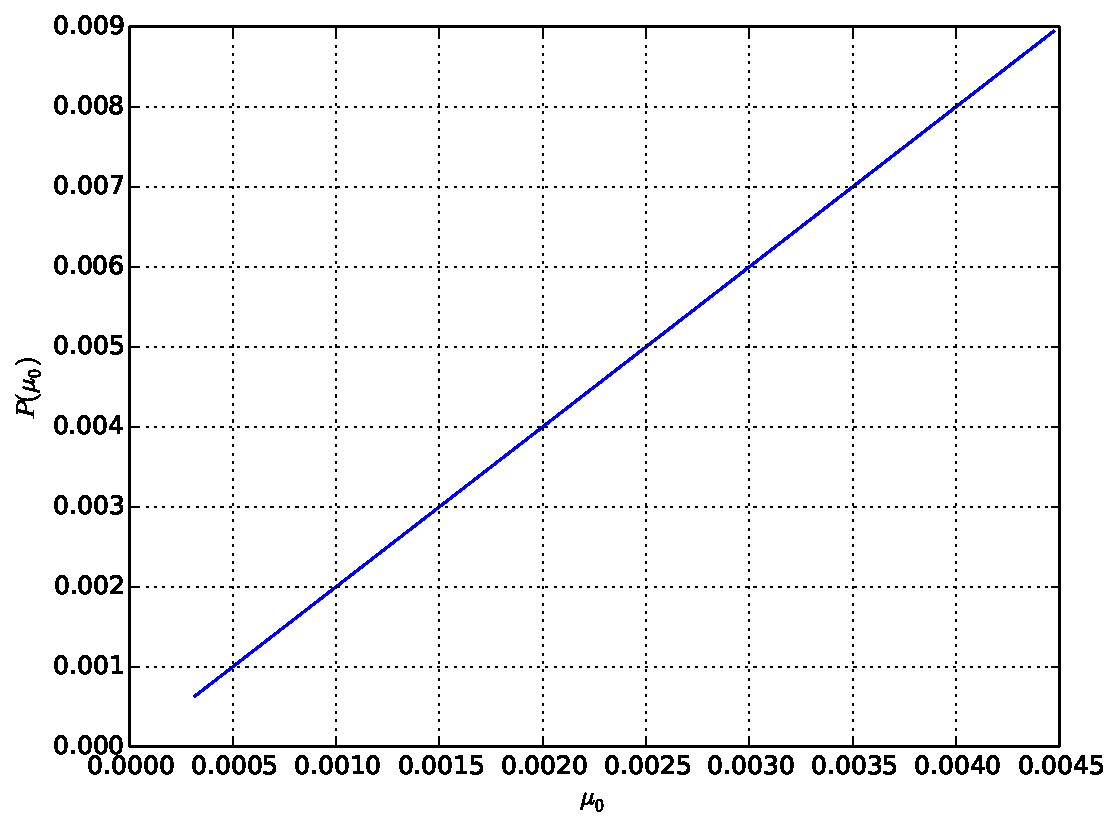
\includegraphics[width=0.5\textwidth]{scat_kernel.pdf}
    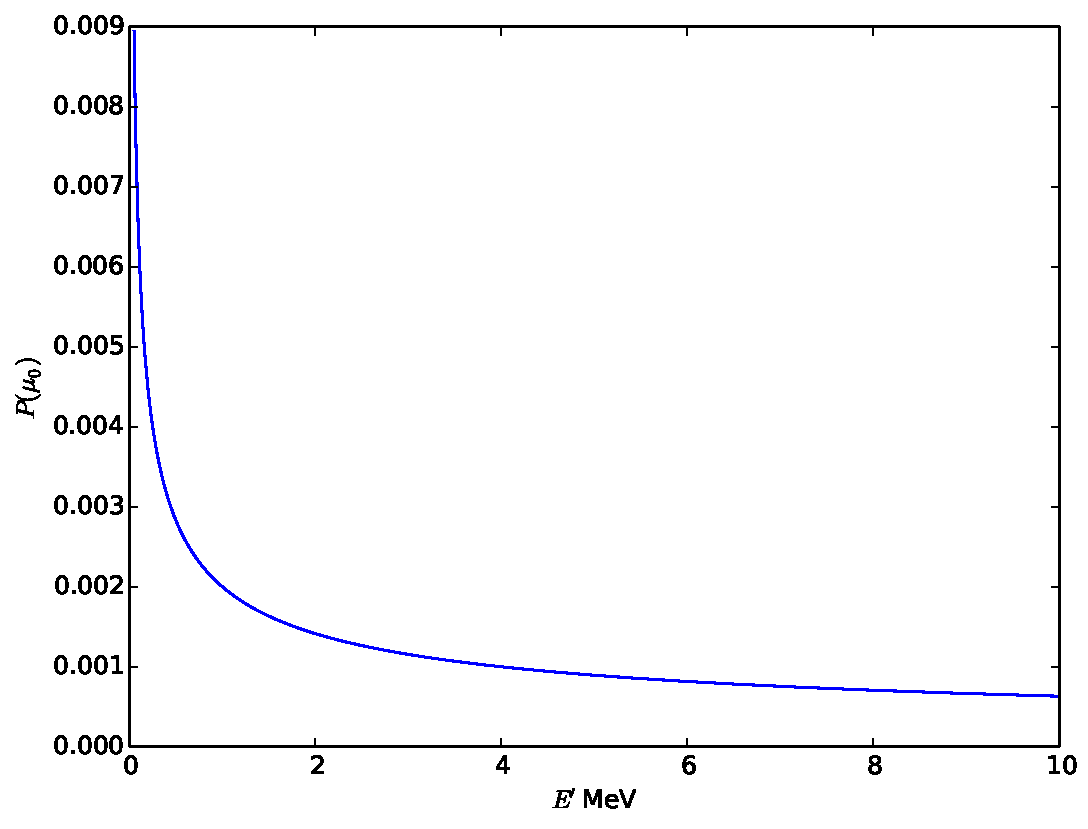
\includegraphics[width=0.5\textwidth]{scat_kernel_E.pdf}
\end{figure*}

 




 \end{solution}

 \begin{thebibliography}{9}

     \bibitem{dunnshultis}
         W.L. Dunn and J.K. Shultis, \emph{Exploring Monte Carlo Methods}, 2012.


\end{thebibliography}

\end{document}



